\chapter{Reduced Electronic Density Distribution} \label{ED}

A heterojuntion is basically a p-n junction in a semiconductor between
materials of different composition. Normal junctions are between p and n type
versions of the same material. But in this case we refer to a juntion formed
betewen two group III-arsenide usually a GaAs/AlAs interface or a GaAs/AlGaAs
interface. Since they are two differnt materials, the band structure is
discontinuous from one material to the other and the band alignment across the
interface is typically of type I, i.e. the band gap of the lower bandgap
material is positioned energetically within the bandgap of the wider bandgap
semiconductor.

Polarization fields 
The usual growth direction for hexagonal III-V materials is
along the polar [0001] axis, for which the crystal lacks inversion symeetry.
This will result in the formation of polarization fields. There are two kinds
of polarization fields. They are spontaneous polarization (SP) and
Piezoelectric polarization (PZ).  The spontaneous polarization exists in polar
semiconductors with a Wurzite or lower symmetry crystal structure and is
related to the deviation of the crystal lattice parameters from the ideal
values for the structure, thereby creating molecular dipoles in the material
building a polarization field just like that formed in ferroelectrics. This
field has a fixed direction along the [0001] c-axis in the Wurtzite lattice.
Therefore the field resulting from spontaneous polarization will point along
the growth direction and this maximizes pontaneous polarization effect in these
systems and renders the problem effectively one-dimensional.  

The other type of polarization field, the piezoelectric polarization occurs due
to the presence of strain in the system. When two layers are joined together to
form a heterojunction, the difference in the lattice constant between the two
materials will lead to a strain . This strain also occurs due tot he difference
in the thermal expansion coefficients in the the layers during cool down after
growth. This leads to elastic strain in the layers. 

\section{Self-consistent Poisson-Schrodinger Solver} \label{sec:model}

The study of energy band structures of heterostructures needs a detailed
knowledge of optical and transport properties of the heterostructures. These
properties can be found by solving sefl-consistently Poisson's and
Schrodinger's equations for the elctron wave functions.

The finite difference method (FDM) is a simple and efficient method for solving
ordinary differential equations (ODEs) in problem regions with simple
boundaries. FDM can be used to solve for the Schrodinger equation. The method
requires the construction of a mesh defining local coordinate surfaces. For
each node of this mesh, the unknown function values are found, replacing the
differntial equations by difference equations. These values gives the vector
solution for $\phi$ and a matric formulation if the Schrodinger equation.
where A is the matrix operator and $\lamda$ the energy eigenvalues. Usually a
uniform mesh size is selected but this means that this method is not effective.
Need a small mesh when the wavefunction is changing rapidly and a large mesh
during a slow change in the wavefunction for the ideal speed. Moreover, careful
calculations are also required at the juntion of two different mesh sizes and
destroying the symmetry of the matrix A, making it more difficult to calculate. 
%\subsection{What Reddening Law Fits Better?}\label{sec:DIC}


\section{Electronic Distribution in Nanowires} \label{sec:spectra}

Figure 8 (C) shows the FDTD-simulated electric field density of a hexagonal
nanowire at y cross section (top) and x cross section (bottom). The photon
energy of this mode shown as the insets of Fig. 8(C) is concentrated primarily
along the 6 corners and secondarily along the facets with little light in the
3D core of GaAs. Hence, we suggest that the fortuitous spatial overlap of the
resonant optical modes on reduced dimensional electronic wavefunctions plays a
significant role in the remarkable optoelectronic properties of core-shell
nanowires. Restated, the superposition of the photon modes  on reduced
electronic states that form on the facets and vortices of the hexagonal CSNWs
strongly enhances both upward and downward transition rates.  Thus, the reduced
dimensionality transition rate distinguishes the core-shell nanostructure from
the optically equivalent structures of Fig. 6 due to its significantly modified
rate management. These nanostructures are not only excellent optical cavities,
but despite their large size also provide the right reduced dimensional
electronic structures which enhance optoelectronic interactions.  It should be
noted the present analysis is for direct optical transitions; although it can
be extended to incorporate k-vector changes as in phonon scattering, other
important factors such as many-body interactions need to be included in a
comprehensive analysis.

\subsection{Cylindrical Core-Shell Nanowire}

\subsection{Hexagonal Core-shell Nanowire} \label{sec:indv_lines}

\begin{figure}
  \caption{One Dimensional Electron Charge with band bending}
  \centering
  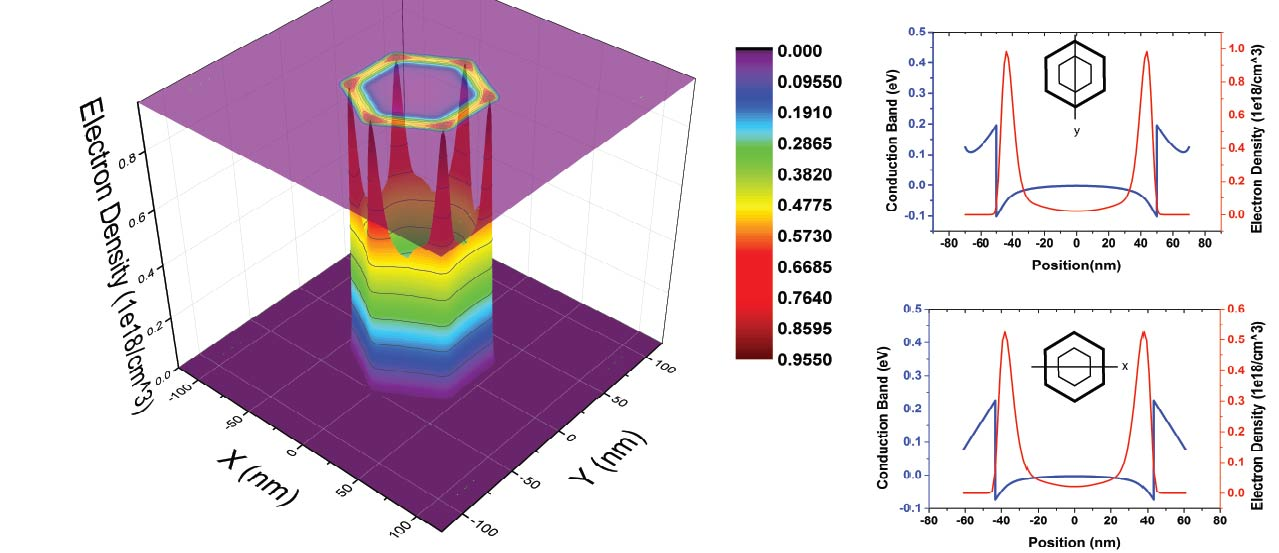
\includegraphics[width=\textwidth]{pictures/ED/1DCharge}
  \label{1DCharge}
\end{figure}

\begin{figure}
  \caption{Two Dimensional Electron Charge with band bending}
  \centering
  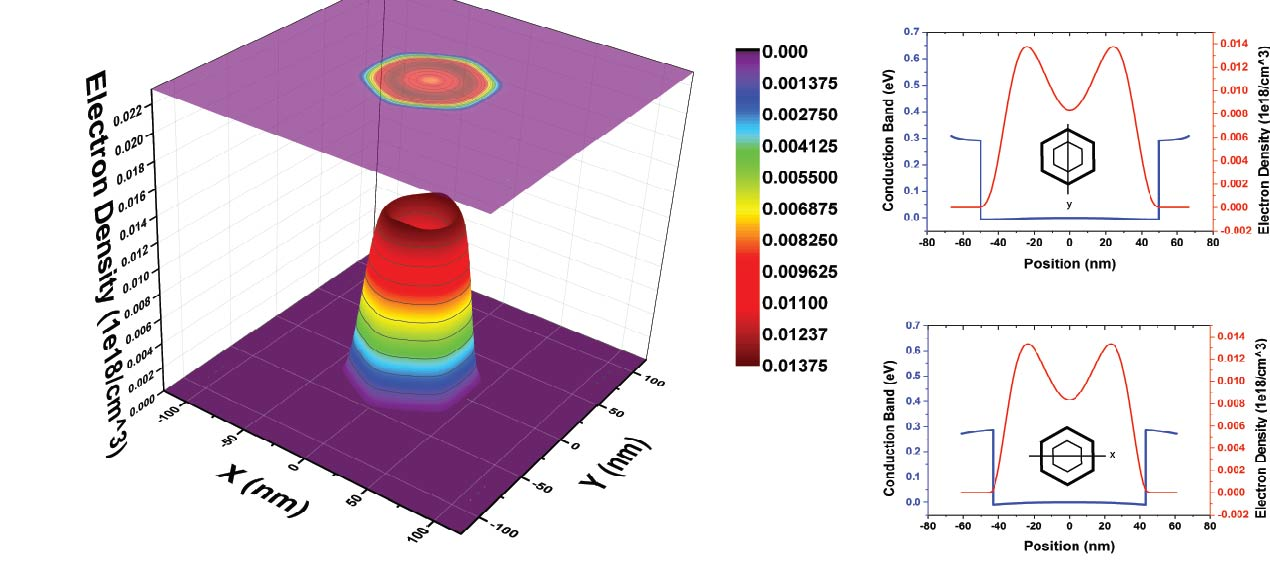
\includegraphics[width=\textwidth]{pictures/ED/2DCharge}
  \label{2DCharge}
\end{figure}

\begin{figure}
  \caption{Three Dimensional Electron Charge with band bending}
  \centering
  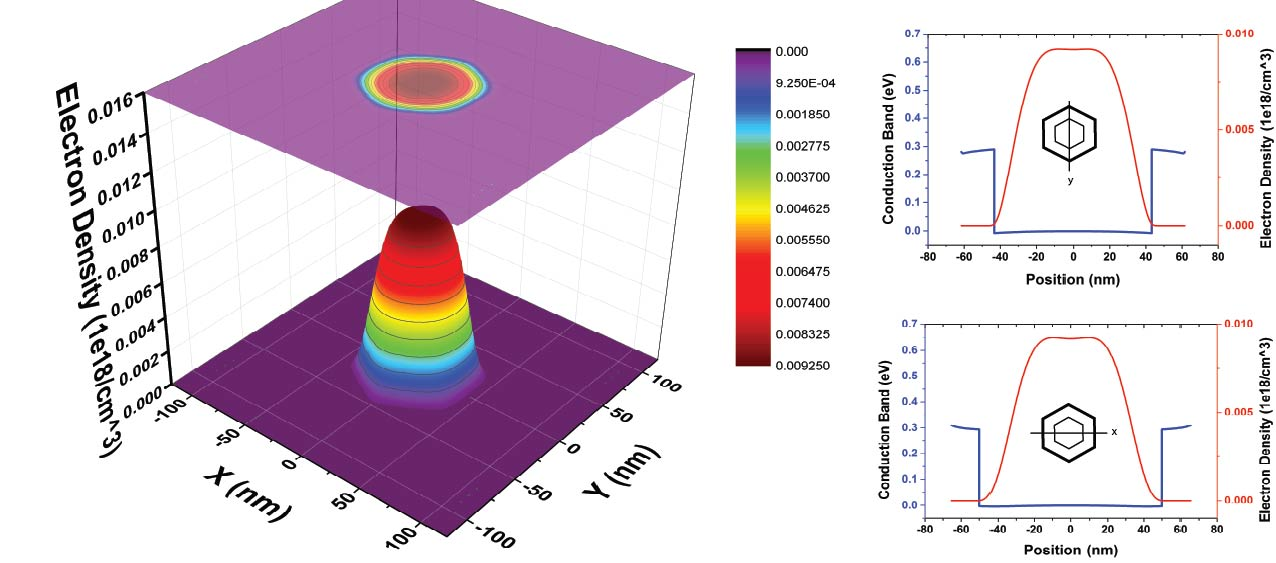
\includegraphics[width=\textwidth]{pictures/ED/3DCharge}
  \label{3DCharge}
\end{figure}

\begin{figure}
  \caption{Photon Charge Distribution}
  \centering
  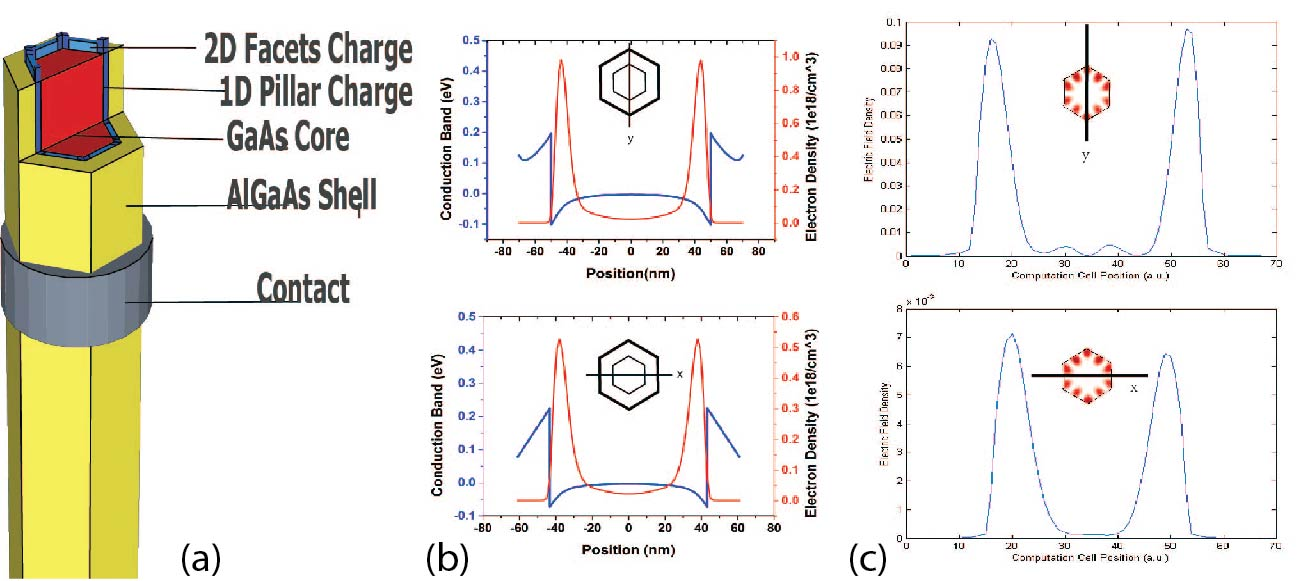
\includegraphics[width=\textwidth]{pictures/ED/Photoncharge}
  \label{PhotonCharge}
\end{figure}

\section{Conclusions} \label{sec:conclusions}

